\documentclass[aspectratio=169]{beamer}

\usetheme{default}  % You can choose any other theme you prefer

\title{My Presentation}
\author{Your Name}
\date{\today}

\usepackage{tikz}

\begin{document}

\begin{frame}
\titlepage
\end{frame}

\section{Introduction}
\begin{frame}
\frametitle{Introduction}
This is the introduction slide.
\end{frame}

\section{Main Content}
\begin{frame}
\frametitle{Main Content}
This is a slide in the main content section.
\end{frame}

\section{Visualization}
\begin{frame}
\frametitle{2D Plane Division}
\begin{center}
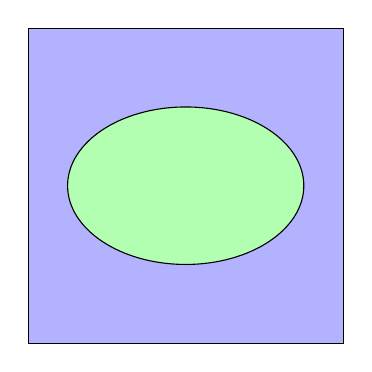
\begin{tikzpicture}
  \fill [blue!30] (-2,-2) rectangle (2,2) node[midway] (omega_up) {$\Omega_{\text{up}}$};
  \fill [green!30] (0,0) ellipse (1.5cm and 1cm) node[midway] (omega_down) {$\Omega_{\text{down}}$};
  \draw (-2,-2) rectangle (2,2);
  \draw (0,0) ellipse (1.5cm and 1cm);
\end{tikzpicture}
\end{center}
\end{frame}

\section{Conclusion}
\begin{frame}
\frametitle{Conclusion}
This is the conclusion slide.
\end{frame}

\end{document}
